\section{Rationale Funktionen}
Eine rationale Funktion ist eine Funktion der Form
\[
    f(x) = \frac{p(x)}{q(x)} = \frac{a_n x^n + a_{n-1} x^{n-1} + \ldots + a_1 x + a_0}{b_m x^m + b_{m-1} x^{m-1} + \ldots + b_1 x + b_0}
\]
wobei \(p(x)\) und \(q(x)\) Polynome sind und \(q(x) \neq 0\).

\subsection{Eigenschaften}
Rationale Funktionen haben folgende Eigenschaften:
\begin{itemize}
    \item Sie sind definiert, solange der Nenner \(q(x)\) nicht null ist.
    \item Sie können durch Partialbruchzerlegung in einfachere Brüche zerlegt werden.
    \item Sie haben höchstens so viele Nullstellen wie der Grad des Zählers.
\end{itemize}

\subsection{Definitionslücken}
Rationale Funktionen können Definitionslücken aufweisen, die auftreten, wenn der Nenner \(q(x)\) an bestimmten Stellen null wird. An diesen Stellen ist die Funktion nicht definiert.

Sei \(x_0\) eine Definitionslücken von \(f(x)\). Der Linearfaktor \((x - x_0)\) sei aus \(p(x)\) und \(q(x)\) abgeteilt:
\[
    f(x) = \frac{(x - x_0)^{j_p} \cdot p_1(x)}{(x - x_0)^{j_q} \cdot q_1(x)}, \quad p_1(x_0), \quad q_1(x_0) \neq 0
\]
mit \(j_p, j_q \in \mathbb{N}\) und \(j_q > 1\).

\begin{itemize}
    \item Wenn \(j_p \le j_q\), dann ist \(x_0\) eine \emph{hebbare} Definitionslücke.
    \item Wenn \(j_p < j_q\), dann ist \(x_0\) eine Polstelle der Ordnung \(j_q - j_p\).
    \begin{itemize}
        \item Ordnung gerade: Polstelle ohne Vorzeichenwechsel.
        \item Ordnung ungerade: Polstelle mit Vorzeichenwechsel.
    \end{itemize}
    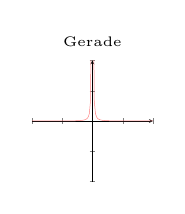
\begin{tikzpicture}[scale=.45]
        \begin{axis}[axis lines=middle, xmin=-2, xmax=2, ymin=-2, ymax=2, width=5cm, height=5cm, yticklabel={\empty}, xticklabel={\empty}]
            \addplot[domain=-2:2, samples=100, red!50] {1/(20*x)^2};
        \end{axis}
      \node[anchor=south] at (current bounding box.north) {\tiny{Gerade}};
    \end{tikzpicture}
    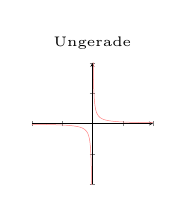
\begin{tikzpicture}[scale=.45]
        \begin{axis}[axis lines=middle, xmin=-2, xmax=2, ymin=-2, ymax=2, width=5cm, height=5cm, yticklabel={\empty}, xticklabel={\empty}]
            \addplot[domain=-2:0, samples=100, red!50] {1/(20*x)};
            \addplot[domain=0:2, samples=100, red!50] {1/(20*x)};
        \end{axis}
      \node[anchor=south] at (current bounding box.north) {\tiny{Ungerade}};
    \end{tikzpicture}
    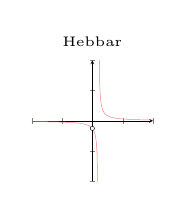
\begin{tikzpicture}[scale=.45]
        \begin{axis}[axis lines=middle, xmin=-2, xmax=2, ymin=-2, ymax=2, width=5cm, height=5cm, yticklabel={\empty}, xticklabel={\empty}]
            \addplot[domain=-2:0.2, samples=100, red!50] {x/(20*x*(x-0.2))};
            \addplot[domain=0.2:2, samples=100, red!50] {x/(20*x*(x-0.2))};
                \node at (axis cs:0,-0.25) [circle, draw=black, fill=white, inner sep=1.2pt] {};
        \end{axis}
      \node[anchor=south] at (current bounding box.north) {\tiny{Hebbar}};
    \end{tikzpicture}
\end{itemize}

\subsection{Asymptoten}
Rationale Funktionen können folgende Asymptoten haben:
\begin{itemize}
    \item \emph{Vertikale Asymptoten}: Treten auf, wenn \(q(x) = 0\) und \(p(x) \neq 0\).
    \item \emph{Horizontale Asymptoten}: Bestimmen das Verhalten von \(f(x)\) für \(x \to \pm \infty\).
    \item \emph{Polynomiale Asymptoten}: Treten auf, wenn der Grad des Zählers grösser ist als der Grad des Nenners. Sie können durch Polynomdivision gefunden werden.
\end{itemize}

\subsection{Graphen}
Der Graph einer rationalen Funktion kann durch Nullstellen und Asymptoten skizziert werden. Dabei sind die Nullstellen die Lösungen von \(p(x) = 0\) und die Asymptoten die Lösungen von \(q(x) = 0\).